\begin{frame}
\end{frame}

\begin{frame}
  \frametitle{Linux与生物信息学}
  \begin{description}
    \item[编程语言] 很多生物信息学软件以C源代码包的形式进行发布,需要编译安装后才能使用;Linux是用C写的
    \item[作业支持] 生物信息的主要工作是用软件和脚本处理生物数据,尤其是生物大数据;Linux稳定、开源、免费,是服务器操作系统的首选,对高性能和大数据的支持好,高性能集群和云平台大多基于Linux
    \item[软件工具] 一般的生物信息分析软件都是基于Linux开发的;Linux中的生物信息软件包和脚本丰富,命令丰富,shell可编程能力强,定制设计和开发容易
    \item[文本处理] 生物信息学数据大多以纯文本进行保存;Linux中开箱即用的文本处理命令丰富、易用、高效
    \item[岗位要求] 生物信息学工作者使用最多的平台就是Linux操作系统;Linux是应聘生物信息学岗位的必备技能之一(Linux,Perl/Python,R,NGS,……)
    \item[脑洞大开] 我专业、我自豪、我骄傲、我懒惰、……
  \end{description}
\end{frame}

\begin{frame}
  \frametitle{Linux与天津地铁(Ubuntu 10.04)}
  \begin{figure}
    \centering
    \includegraphics[width=0.38\textwidth]{c0_linux_railway_01.jpg}\quad
    \includegraphics[width=0.45\textwidth]{c0_linux_10_04.jpg}
  \end{figure}
  \pause
  \begin{block}{如果你是}
    \begin{itemize}
      \item 教师:Linux授课素材
      \item 学生:Linux与日常生活
      \item 政府官员:在保证正常使用的前提下及时维护更新系统
      \item 黑客/骇客:警告/攻击系统,勒索钱财、制造混乱
    \end{itemize}
  \end{block}
\end{frame}

\begin{frame}
  \frametitle{Linux与影视}
  \begin{figure}
    \centering
    \includegraphics[width=0.9\textwidth]{c0_linux_movie_01.jpg}
  \end{figure}
\end{frame}

\begin{frame}
  \frametitle{课程目标}
  \begin{block}{适用对象}
    \begin{itemize}
      \item Linux新手,对Linux感兴趣
      \item Linux菜鸟,扩充Linux知识
      \item 期望应用Linux的生物信息学工作者
    \end{itemize}
  \end{block}
  \pause
  \begin{block}{不适用对象}
    \begin{itemize}
      \item 学习并掌握Linux内核/系统的计算机基础(本课程以应用为主)
      \item 成为Linux高手(修行在个人;唯手熟尔;一万小时定律)
      \item 掌握Linux的所有内容(没有一个人可以做到这一点)
    \end{itemize}
  \end{block}
  \pause
  \begin{block}{课程目标}
    \begin{itemize}
      \item 掌握Linux的基本常识,并能够熟练使用Linux
      \item 能够将Linux应用到日常的生物信息学工作中
    \end{itemize}
  \end{block}
\end{frame}

\begin{frame}
  \frametitle{可能的疑问}
  \begin{block}{两个问题}
  \begin{enumerate}
    \item \textcolor{gray}{【你的疑问】}课程是“Linux系统概论”,教材却是《Unix入门经典》。写错了?
    \item \textcolor{gray}{【我的疑问】}对于Linux,你是闻所未闻,还是“日用而不知”?
  \end{enumerate}
\end{block}
  \pause
  \begin{block}{简单的回答}
  \begin{enumerate}
    \item Linux和Unix的区别:前者免费,后者收费
    \item 口袋里的手机,搜索、网购背后的服务器,……
  \end{enumerate}
\end{block}
\end{frame}

\begin{frame}
  \frametitle{新的视野}
  \begin{center}
    透过窗户(Windows)窥探世界 $\Longrightarrow$ 漫步太空俯瞰全球
  \end{center}
  \vspace{-1em}
  \begin{figure}
    \centering
    \visible<1->{\includegraphics[width=5cm]{c0_windows_view_02.jpg}}
    \quad
    \visible<2->{\includegraphics[width=5.4cm]{c0_linux_view_02.png}}
  \end{figure}
\end{frame}

\begin{frame}
  \frametitle{Linux的世界}
  \begin{figure}
    \centering
    %\includegraphics[width=12cm]{c0_linux_world_04.png}
    \includegraphics[width=12cm]{c0_linux_world_06.jpg}
  \end{figure}
\end{frame}

\begin{frame}
  \frametitle{授课教材}
  \begin{figure}
    \centering
    \includegraphics[width=6cm]{c0_books.png}
  \end{figure}
\end{frame}

\begin{frame}
  \frametitle{课程安排 | 理论课}
  \begin{center}
  \alert{后9周,每周二,下午前两节(13:30-15:10),西楼610}\\
  \vspace{0.2cm}
  {\footnotesize
  \textit{纯英文的幻灯片大部分摘抄自edX上的课程:\\ \href{https://www.edx.org/course/introduction-linux-linuxfoundationx-lfs101x-2}{LinuxFoundationX: LFS101x.2 Introduction to Linux}}
  }
  \end{center}
  \vspace{-0.5cm}
  \begin{table}
    \centering
    \rowcolors[]{1}{blue!20}{blue!10}
    \begin{tabular}{cllcc}
      \hline
      \rowcolor{blue!50}顺序 & 授课内容 & 教材章节 & 学时 & 日期\\
      \hline
      1 & Linux基础 & 第1、2章 & 2 & 4.30\\
      2 & 用户和组 & 第3章 & 2 & 5.7\\
      3 & 文件系统 & 第4章 & 2 & 5.14\\
      4 & Linux命令 & 第6章 & 2 & 5.21\\
      5 & 高级Linux命令 & 第8、9章 & 2 & 5.28\\
      6 & 软件安装 & 第19章 & 2 & 6.4\\
      7 & vi/Vim编辑器 & 第7章 & 2 & 6.11\\
      8 & shell脚本编程(上) & 第13、14章 & 2 & 6.18\\
      9 & shell脚本编程(下) & 第13、14章 & 2 & 6.25\\
      %9 & Perl语言简介 & 第17章 & 2 & 7.07\\
      \hline
    \end{tabular}
  \end{table}
\end{frame}

\begin{frame}
  \frametitle{课程安排 | 实验课}
  \begin{center}
  \alert{后9周,每周四,下午后两节(15:30-17:10),教一楼304}\\
  \vspace{0.2cm}
  {\footnotesize
  \textit{部分实验内容摘抄自:\\ 《Linux基础及应用习题解析与实验指导》(谢蓉\ 编著,第二版,中国铁道出版社)}
  }
  \end{center}
  \vspace{-0.5cm}
  \begin{table}
    \centering
    \rowcolors[]{1}{blue!20}{blue!10}
    \begin{tabular}{cllcc}
      \hline
      \rowcolor{blue!50}顺序 & 实验内容 & 理论知识 & 学时 & 日期\\
      1 & 在虚拟机中安装Linux & Linux基础 & 2 & 5.2\\
      2 & Linux图形界面下的文件操作 & \textcolor{gray}{文件系统} & 2 & 5.9\\
      3 & Linux命令行下的文件操作 & 文件系统 & 2 & 5.16\\
      4 & Linux常用命令操作 & Linux命令 & 2 & 5.23\\
      5 & Linux高级命令操作 & 高级Linux命令 & 2 & 5.30\\
      6 & Linux中软件的安装 & 软件安装 & 2 & 6.6\\
      7 & Vim编辑器的使用 & vi/Vim编辑器 & 2 & 6.13\\
      8 & shell脚本的编写(上) & shell脚本编程(上) & 2 & 6.20\\
      9 & shell脚本的编写(下) & shell脚本编程(下) & 2 & 6.27\\
      %9 & Perl脚本的编写 & Perl语言简介 & 2 & 7.09\\
      \hline
    \end{tabular}
  \end{table}
\end{frame}

\begin{frame}
  \frametitle{考核方式}
  \begin{enumerate}
    \item 理论课:60\%
      \begin{enumerate}
        \item 平时表现:10\%
        \item 闭卷考试:50\%
      \end{enumerate}
    \item 实验课:40\%
      \begin{enumerate}
        \item 平时表现:20\%
        \item 实验报告:20\%
      \end{enumerate}
  \end{enumerate}
\end{frame}

